\section{Introduction}
\nblink{brats/12\_rise\_masks.ipynb}

The results from applying RISE on our segmentations problems (BraTS and testnet) where underwhelming. While they showed a low resolution heat map output on both tasks,
on the testnet is missed out a big part (the right side of the image) which is very important for the correct generation of the segmentation output.

We suspect that this is caused by the low information entropy retained after applying a RISE mask on an image, as shown in Figure \ref{hdm_rise_mask}.
The basic idea of occluding a part of an image is not new and has been proposed by Zeiler et. al. in 2014 \cite{zeiler2014visualizing} in a highly cited paper.
Another similar method is Prediction Difference Analysis \cite{zintgraf2017visualizing} by Zintgraf et al.

Still, all investigated algorithms and methods were originally built for image classification tasks. We therefore propose a new method based on the same basic idea
of occluding parts of an image to see how it changes the output, but in a way that is specialized for image segmentation tasks.

\begin{figure}[H]
    \centering
    \begin{subfigure}[t]{.32\textwidth}
        \centering
        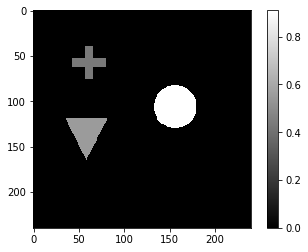
\includegraphics[width=\linewidth]{chapters/02_methods/images/rise/rise_original.png}
        \caption{Original image}
    \end{subfigure}\hfill%
    \begin{subfigure}[t]{.32\textwidth}
        \centering
        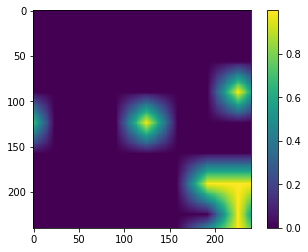
\includegraphics[width=\linewidth]{chapters/02_methods/images/rise/rise1_mask.png}
        \caption{RISE mask}
    \end{subfigure}\hfill%
    \begin{subfigure}[t]{.32\textwidth}
        \centering
        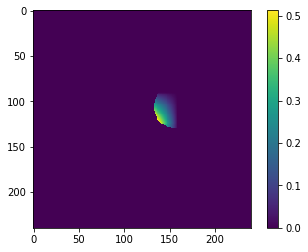
\includegraphics[width=\linewidth]{chapters/02_methods/images/rise/rise1_applied.png}
        \caption{RISE mask applied to original image by multiplication}
    \end{subfigure}
    \caption{By multiplication the input image (left) with a RISE mask (center), a modified input is generated (right).}
    \label{hdm_rise_mask}
\end{figure}
